%==============================================================
\chapter{PROJECT METRICS}
\label{ch:metrics}
%==============================================================

\section{Challenges Faced}
\tabref{tab:challenges} lists the main challenges the team met and how each was addressed. The first two---false alarms in a room the models had never seen, and building a labelled dataset of its own---shaped the project more than any other.
\begin{table}[H]
\caption{Main challenges and how they were addressed}
\label{tab:challenges}
\centering\tablefont
\begin{tabularx}{\textwidth}{|L{4.2cm}|Y|}
\hline\rowhead
\thead{Challenge} & \thead{How it was addressed}\\ \hline
False alarms in a room the models had never seen (about 171 weapon episodes per hour in the first live run) & Diagnosed from the replayable event log; confirmation, person gate, corroboration and per-room thresholds; measured by committed level\\ \hline
No public footage of the threats in a home like ours: the team staged, filmed and labelled its own scenes & Frame-by-frame review, splits by video, LOVO selection, a pre-registered bar, experimental classes capped at Level~2, and a recording feature to collect deployment-room data\\ \hline
A video preview at 0.6\,fps and a 3\,s tick on a 24-thread laptop & Found ONNX Runtime spin-waiting and a blocking capture loop; separate capture, inference, identity and preview threads\\ \hline
A transformer backbone on a four-core board & 4\,s clip engine with a stage cascade, ONNX, 320\,px object stage and a fast lane; slim CNNs tried and rejected under a fixed protocol\\ \hline
Aligning sound with video and telling a fight from play & Time-stamped audio windows that vote only when aligned, non-overlapping fresh windows, background and banter cues\\ \hline
A safe alert flow without a real monitoring centre & The SENTRIX Desk as a simulated responder, test mode with an allowlist, a send guard on every message, and tests that cannot send\\ \hline
WhatsApp business set-up out of reach for students & Switched the demonstration to the already-built Telegram channel; WhatsApp kept in the code\\ \hline
Raspberry~Pi~5 specifics (no RPi.GPIO, CSI camera not in OpenCV, PipeWire audio) & gpiozero with lgpio, Picamera2, ALSA \code{plughw} with resampling; a doctor tool that checks each\\ \hline
Many parallel workstreams & A written contract and eight tracks in separate worktrees, merged in order with integration notes and an end-to-end suite\\ \hline
\end{tabularx}
\end{table}

\section{Relevant Subjects}
\tabref{tab:subjects} maps the subjects of the curriculum to the parts of SENTRIX where they were applied.
\begin{table}[H]
\caption{Subjects of the curriculum applied in the project}
\label{tab:subjects}
\centering\tablefont
\begin{tabularx}{\textwidth}{|L{4.4cm}|Y|}
\hline\rowhead
\thead{Subject} & \thead{Where it was applied}\\ \hline
Machine Learning and Deep Learning & Fine-tuning DINOv2 and YOLO heads, calibration, cross-validation, ROC analysis\\ \hline
Computer Vision / Image Processing & Detection, tracking, keyframe selection, motion energy, perceptual hashing\\ \hline
Signals and Systems / Digital Signal Processing & Resampling with anti-alias filtering, log-mel spectrograms, audio windows\\ \hline
Probability and Statistics & Poisson and Clopper--Pearson intervals, threshold selection, score distributions\\ \hline
Operating Systems & Threads and queues, systemd services and watchdogs, process isolation\\ \hline
Computer Networks & WebSockets, outbound links, tunnelling, NAT and firewalls, a hosted cloud service\\ \hline
Database Management Systems & SQLite schemas and migrations, write-ahead logging, Postgres compatibility\\ \hline
Software Engineering & Requirements (SRS), contracts, test plans, reviews, version control\\ \hline
Information Security and Cryptography & AES-GCM, HKDF, SHA-256 hash chains, Argon2id, TOTP, CSP and CSRF\\ \hline
Embedded Systems / IoT & GPIO, status LEDs, the Pi camera, a USB microphone, node telemetry and the systemd watchdog\\ \hline
Web Technologies & FastAPI, React, TypeScript, accessible UI design\\ \hline
Engineering Design & Enclosure CAD, interference checks, bill of materials and cost analysis\\ \hline
\end{tabularx}
\end{table}

\section{Interdisciplinary Knowledge Sharing}
The project required knowledge well beyond computer science, and members taught each other as each area came up. \textbf{Electronics:} LED drive through current-limiting resistors on 3.3\,V GPIO pins, and the Pi's power and current limits (why the official 27\,W supply). \textbf{Mechanical design:} a parametric enclosure from the manufacturer's mechanical drawings, tolerances for 3D printing and a tilting camera pod. \textbf{Acoustics:} microphone sample rates, aliasing, and how television, laughter and shouting differ in a tagger's labels. \textbf{Law and ethics:} consent of everyone filmed, the DPDP Act's consent, notice and erasure duties, and never contacting emergency services automatically. \textbf{Human factors:} what a frightened person can do on a phone, accessible contrast and touch targets, plain-language copy, and a duress path. \textbf{Operations:} cloud hosting, cost control, and deployment on a headless device.

\section{Peer Assessment Matrix}
Each member rates the contribution of every member, including themselves, from 1 (minimum) to 5 (maximum). The ratings are entered by the members at submission (\tabref{tab:peer}).

\begin{table}[H]
\caption{Peer assessment matrix (ratings 1--5)}
\label{tab:peer}
\centering\tablefont
\renewcommand{\arraystretch}{1.6}
\begin{tabular}{|c|l|C{1.5cm}|C{1.5cm}|C{1.5cm}|C{1.5cm}|C{1.5cm}|}
\cline{3-7}
\multicolumn{2}{c|}{} & \multicolumn{5}{c|}{\textbf{Evaluation of}}\\ \cline{3-7}
\multicolumn{2}{c|}{} & S1 & S2 & S3 & S4 & S5\\ \hline
\multirow{5}{*}{\rotatebox{90}{\textbf{Evaluation by}}} & S1 & & & & & \\ \cline{2-7}
 & S2 & & & & & \\ \cline{2-7}
 & S3 & & & & & \\ \cline{2-7}
 & S4 & & & & & \\ \cline{2-7}
 & S5 & & & & & \\ \hline
\end{tabular}

\vspace{4pt}
{\footnotesize S1: Kartik Garg (102303478), S2: Akshay Ranveer (102303453), S3: Prashant Gagneja (102353011), S4: Harshit Mishra (102319039), S5: Mehul Perimal (102315144).}
\end{table}

\section{Role Playing and Work Schedule}
\tabref{tab:roles} lists the role each member played and \figref{fig:gantt} the schedule of the semester, taken from the project's version-control history. The proposal was approved in March 2026; the mid-semester report was submitted in August 2026.

\begin{table}[H]
\caption{Roles played by the team members}
\label{tab:roles}
\centering\tablefont
\begin{tabularx}{\textwidth}{|L{3.0cm}|L{4.0cm}|Y|}
\hline\rowhead
\thead{Member} & \thead{Role} & \thead{Responsibilities}\\ \hline
Kartik Garg & Vision and backend lead & Architecture, detector path, confirmation rules, YOLO heads\\ \hline
Akshay Ranveer & Identity lead & Faces, tracking, enrolment, body re-identification\\ \hline
Prashant Gagneja & Audio lead & Microphone path, sound model, audio data\\ \hline
Harshit Mishra & Behaviour and fusion lead & Recording protocol, deployment-room data, fusion rules\\ \hline
Mehul Perimal & Records, interfaces and evaluation lead & Incidents, evidence vault, dashboards, evaluation and gate tooling\\ \hline
All members & Testers and demonstrators & Recording sessions, rehearsals, reviews; in the demonstration: owner, emergency contact, Desk operator and device administrator\\ \hline
\end{tabularx}
\end{table}

\begin{figure}[htbp]
\centering
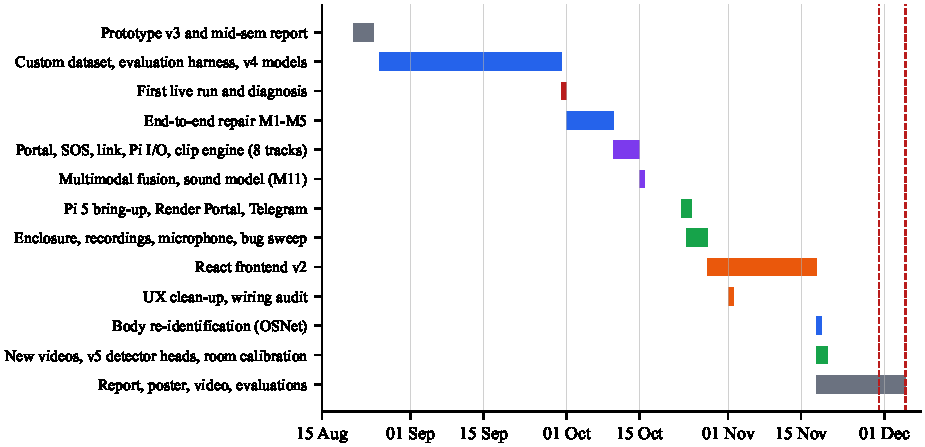
\includegraphics[width=\textwidth]{figures/fig_gantt.pdf}
\caption{Work schedule, August--December 2026 (dashed lines: evaluation on 30 November and final panel on 5 December)}
\label{fig:gantt}
\end{figure}

\section{Student Outcomes Description and Performance Indicators}
\tabref{tab:so} maps each student outcome and performance indicator of the course to the work in this project that demonstrates it.

\begingroup\tablefont
\begin{longtable}{|C{0.9cm}|L{5.5cm}|L{6.8cm}|}
\caption{SO1--SO7 mapping for the course UCS794 Capstone Project}\label{tab:so}\\
\hline\rowhead
\thead{SO} & \thead{SO Description} & \thead{Outcome}\\ \hline
\endfirsthead
\hline\rowhead
\thead{SO} & \thead{SO Description} & \thead{Outcome}\\ \hline
\endhead
\multicolumn{3}{r}{\footnotesize\itshape continued on next page}\\
\endfoot
\endlastfoot
1.1 & Ability to identify and formulate problems related to the computational domain & Identified that home alarms fail through false alarms, cloud dependence and lack of owner control, and formulated detection as committed alarm levels with measurable false-onset rates.\\ \hline
1.2 & Apply engineering, science and mathematics to obtain analytical, numerical and statistical solutions & Defined the evidence and TCI formulas, used Poisson and Clopper--Pearson bounds, ROC analysis and temperature scaling to choose and judge models.\\ \hline
2.1 & Design computing systems to address needs and build prototypes that meet design specifications & Designed and built the device, Portal, two web apps and the Pi~5 unit with enclosure against a written SRS and contract.\\ \hline
2.2 & Ability to analyse the economic trade-offs in computing systems & Compared edge and cloud inference costs, Pi 8\,GB vs 4\,GB, slim vs large models, and hosting options (Render vs Oracle).\\ \hline
3.1 & Prepare and present documents according to computing standards and protocols & Produced nine specifications, a decision log, an SRS following ISO/IEC/IEEE 29148, test documentation following 29119-3, and this report with IEEE references.\\ \hline
3.3 & Communicate effectively with peers using technical knowledge & Coordinated eight parallel tracks through a shared contract, code reviews and integration notes.\\ \hline
4.1 & Aware of ethical and professional responsibilities in computing solutions & Test mode by default, no automatic call to 112, consent of everyone filmed, data kept on the device, honest reporting of limits.\\ \hline
4.3 & Evaluate solutions considering environmental, societal and economic contexts & Assessed privacy under the DPDP Act, the societal cost of false alarms, energy of edge vs cloud, and the cost to a household.\\ \hline
5.1 & Participate in the development and selection of ideas to meet objectives & Proposed and compared fusion approaches, slim models and hardware platforms, selecting them by pre-registered criteria.\\ \hline
5.2 & Plan, share and execute task responsibilities in a team & Split work by subsystem and by track with clear ownership and milestones (M1--M11).\\ \hline
6.1 & Perform experimentation and analyse the results & Ran LOVO cross-validation, video replays, live and Pi benchmarks and re-identification experiments.\\ \hline
6.2 & Analyse and interpret data, make judgements and draw conclusions & Interpreted the room's score distributions to set thresholds, rejected the slim heads and the 0.50 re-id bar on evidence.\\ \hline
7.1 & Explore and utilise resources to enhance self-learning & Learned DINOv2, PANNs, OSNet, Picamera2, gpiozero, React and cloud deployment from papers, datasheets and documentation.\\ \hline
\end{longtable}
\endgroup

\section{Brief Analytical Assessment}
SENTRIX is a working end-to-end prototype of the product. Some items are still open: one interface defect (TC-29), Telegram delivery from the Render Portal to re-check, two release gates (G2, G4), and the Pi's 2\,s latency target. Its strongest results are in the system around the models: the evidence rules removed every false onset at Level~3 and above from the replayed live session and the labelled videos; the assistance flow handles the owner who approves, declines, is coerced or cannot answer; and the device keeps private data at home while the owner keeps control from anywhere. Its measured detection---9 of 12 handgun episodes and all flames at Level~3---comes from the team's own staged recordings, partly from training videos, and the false-alarm rate is bounded only loosely by the normal footage replayed so far, so it is evidence of feasibility rather than a validated rate. On the Raspberry~Pi~5 the product runs end to end but decides in about 4\,s rather than 2\,s. The project's main analytical contribution is its method: every claim is produced by a tool from committed data, model choices are fixed before they are tested, and limits are reported alongside results. The path to a validated product is clear: deployment-room recordings, a single detector trained on them, a fitted fusion model from real verdicts, and a hardware accelerator for the Pi.
